\resetfigpath{dec}

\chapter{A Deep Embedded Clustering approach}
This chapter presents an approach whose ambition is to improve on two components of the previous chapter, namely
(1) The pairwise similarity model that intervenes in the frame-to-frame likelihood model, and
(2) The feature extraction method that intervenes in the foreground prediction model.
In particular, we aimed at generating pairwise similarity labels that would serve to train a pairwise similarity metric, as can be found, for example, in the deep siamese network for multiple object tracking of \cite{cuan18}, or the deep cosine metric learning of \cite{wojke18}.
In our scenario, pairwise similarity labels are not available, which therefore justifies a preliminary self-supervised approach to generate them.
This self-supervised task relies on the \gls{dec} approach, which devises a training scheme that
alternates between a cluster assignment step and centroid update step, similar in spirit to the K-mean algorithm, while the features corresponding to these samples are obtained from the bottleneck of a \gls{cnn} and optimized jointly with the clustering objective.

As will be shown in our experiments, this approach proved to be ineffective in practice, as the above task is very hard to achieve.
In particular, we observed a high sensitivity to a number of hyper-parameters that made the learning process unstable.
The learning rate, the update period of centroids, and the initial values of clusters were tightly dependent, often bringing the learning process to a degenerate solution.
Next, assuming that the above went smoothly, our pairwise similarity module would often bring negligible improvements.
Concretely, several strategies were implemented, namely a siamese network, a cosine similarity metric learning, and a \gls{gmm}.
Neither provided significant improvements to our baseline models.
We therefore chose to present results using the simpler \gls{gmm}.

Despite these negative results, we chose to provide here our general approach for future reference.

\section{Introduction}
\label{sec:intro}

Object segmentation and detection in video and 3D image modalities are crucial problems in medical imaging.
From brain tumors imaged with MRI to surgical instruments in laparoscopic video sequences, supervised machine learning has provided reliable detection and segmention of structures of interest in various medical applications~\cite{menze15,sznitman2014,zikic2014}.
To ensure good prediction performances, a cornerstone of most recent methods and in particular of deep learning methods, is the need for vasts amounts of images and annotations to optimize large numbers of machine learning model parameters. 

Furthermore, while video and 3D image data is increasingly available, generating
ground truth annotations still remains one of the greatest bottlenecks
for creating truly large training datasets. Methods to reduce the annotation
burden have mainly centered on active learning~\cite{KonSznFua15,MosSzn16},
domain adaptation~\cite{ShiRoth16,BerBecSalFua2016} and
crowd-sourcing~\cite{Cheplygina2016}, allowing experts and
non-experts to provide annotations in limited amounts or in parallel. Yet, the
process of providing pixel-wise segmentation ground truth data remains prohibitively slow and tedious regardless. 

In this work, we look to alleviate this burden by proposing a novel method that relies on point-wise, or clicks, annotations of objects of interest.
In this context, a number of methods have been introduced to infer segmentations from sparse 2D annotations in video and 3D volumes.
The work in~\cite{vilarino07} introduced a patch-based SVM within a transductive learning approach to produce segmentations when viewing endoscopy video sequences.
Similarly, \cite{khosravan16} used a gaze tracker to annotate CT volumes with a saliency map-construction and a Random-Walker to segment the object of interest.
An alternative was also presented in~\cite{lejeune17} where an expected exponential loss was used within a Positive-Unknown (PU) learning setting.
In~\cite{bearman16}, a deep learning based approach with point location supervision was used to train a CNN with strong object priors, whereby showing good performances on natural images.
Last, the method introduced in~\cite{lejeune18} relied on multiple instance tracking using limited point-wise supervision showed good generalization on several types of image modalities and objects.
However, this approach suffers several limitations including (i) that the learning of segmentation features are decoupled from the similarity metric used in the tracking optimization and (ii) the use of a superpixel similarity measure is taken as a simple Gaussian distance in the feature space, whereby ignoring potential presence of sub-clusters in the learned latent space.
Both of these negatively impact the performance of the multiple instance tracking and lead to sub-optimal object segmentations. 

To overcome the previously mentioned limitations, we present in this work a novel approach that leverages the assumption that data volumes or sequences are composed of a number of clusters characterezing homogenous regions in the image space. By doing so, our method estimates and refines clusters so to have low intra-variance and high inter-variance in a fully self-supervised fashion~\cite{xie15}. By then simultaneously learning an efficient feature representation and set of clusters (and associations), we use the latter to initialize a Gaussian Mixture Model to model the pairwise similarity of superpixel regions. We show that our approach leads to improved segmentation from point-wise annotations for a wide range of object types across different imaging modalities (video and volumetric) by comparing it to several existing methods. 

%%% Local Variables:
%%% mode: latex
%%% TeX-master: "00_main"
%%% End:

\section{Method}
\label{sec:method}
We begin by introducing some notation and giving a brief overview of the multiple-instance tracking method introduced in \cite{lejeune18} that will serve as the base framework of this work. We then present our approach and highlight its integration in this framework.

\subsection{Base Framework}
The framework operates with a pre-segmentation of the image using standard superpixels~\cite{achanta12} and assumes that each given 2D-point annotation indicates a location on the object of interest. By optiziming a max-flow graph (see Fig.~\ref{fig:ksp_network}), the entire sequence of images can be segmented from point-wise annotations. In \cite{lejeune18}, the annotations are used to model the likelihoods (costs) associated to the red, blue, and green edges of Fig.~\ref{fig:ksp_network}. In particular, two key models are to estimate these costs: (1) a transductive foreground model (blue arrows) and (2) a pairwise probability mode (red and green arrows). The full segmentation is then formulated as a Maximum a posteriori (MAP) problem, cast into a network flow problem, and solved using the edge-disjoint K-shortest paths algorithm \cite{berclaz11}; the latter being a multiple-instance tracking solver. We now detail both below (1) and (2):
\begin{figure}[t]
\centering
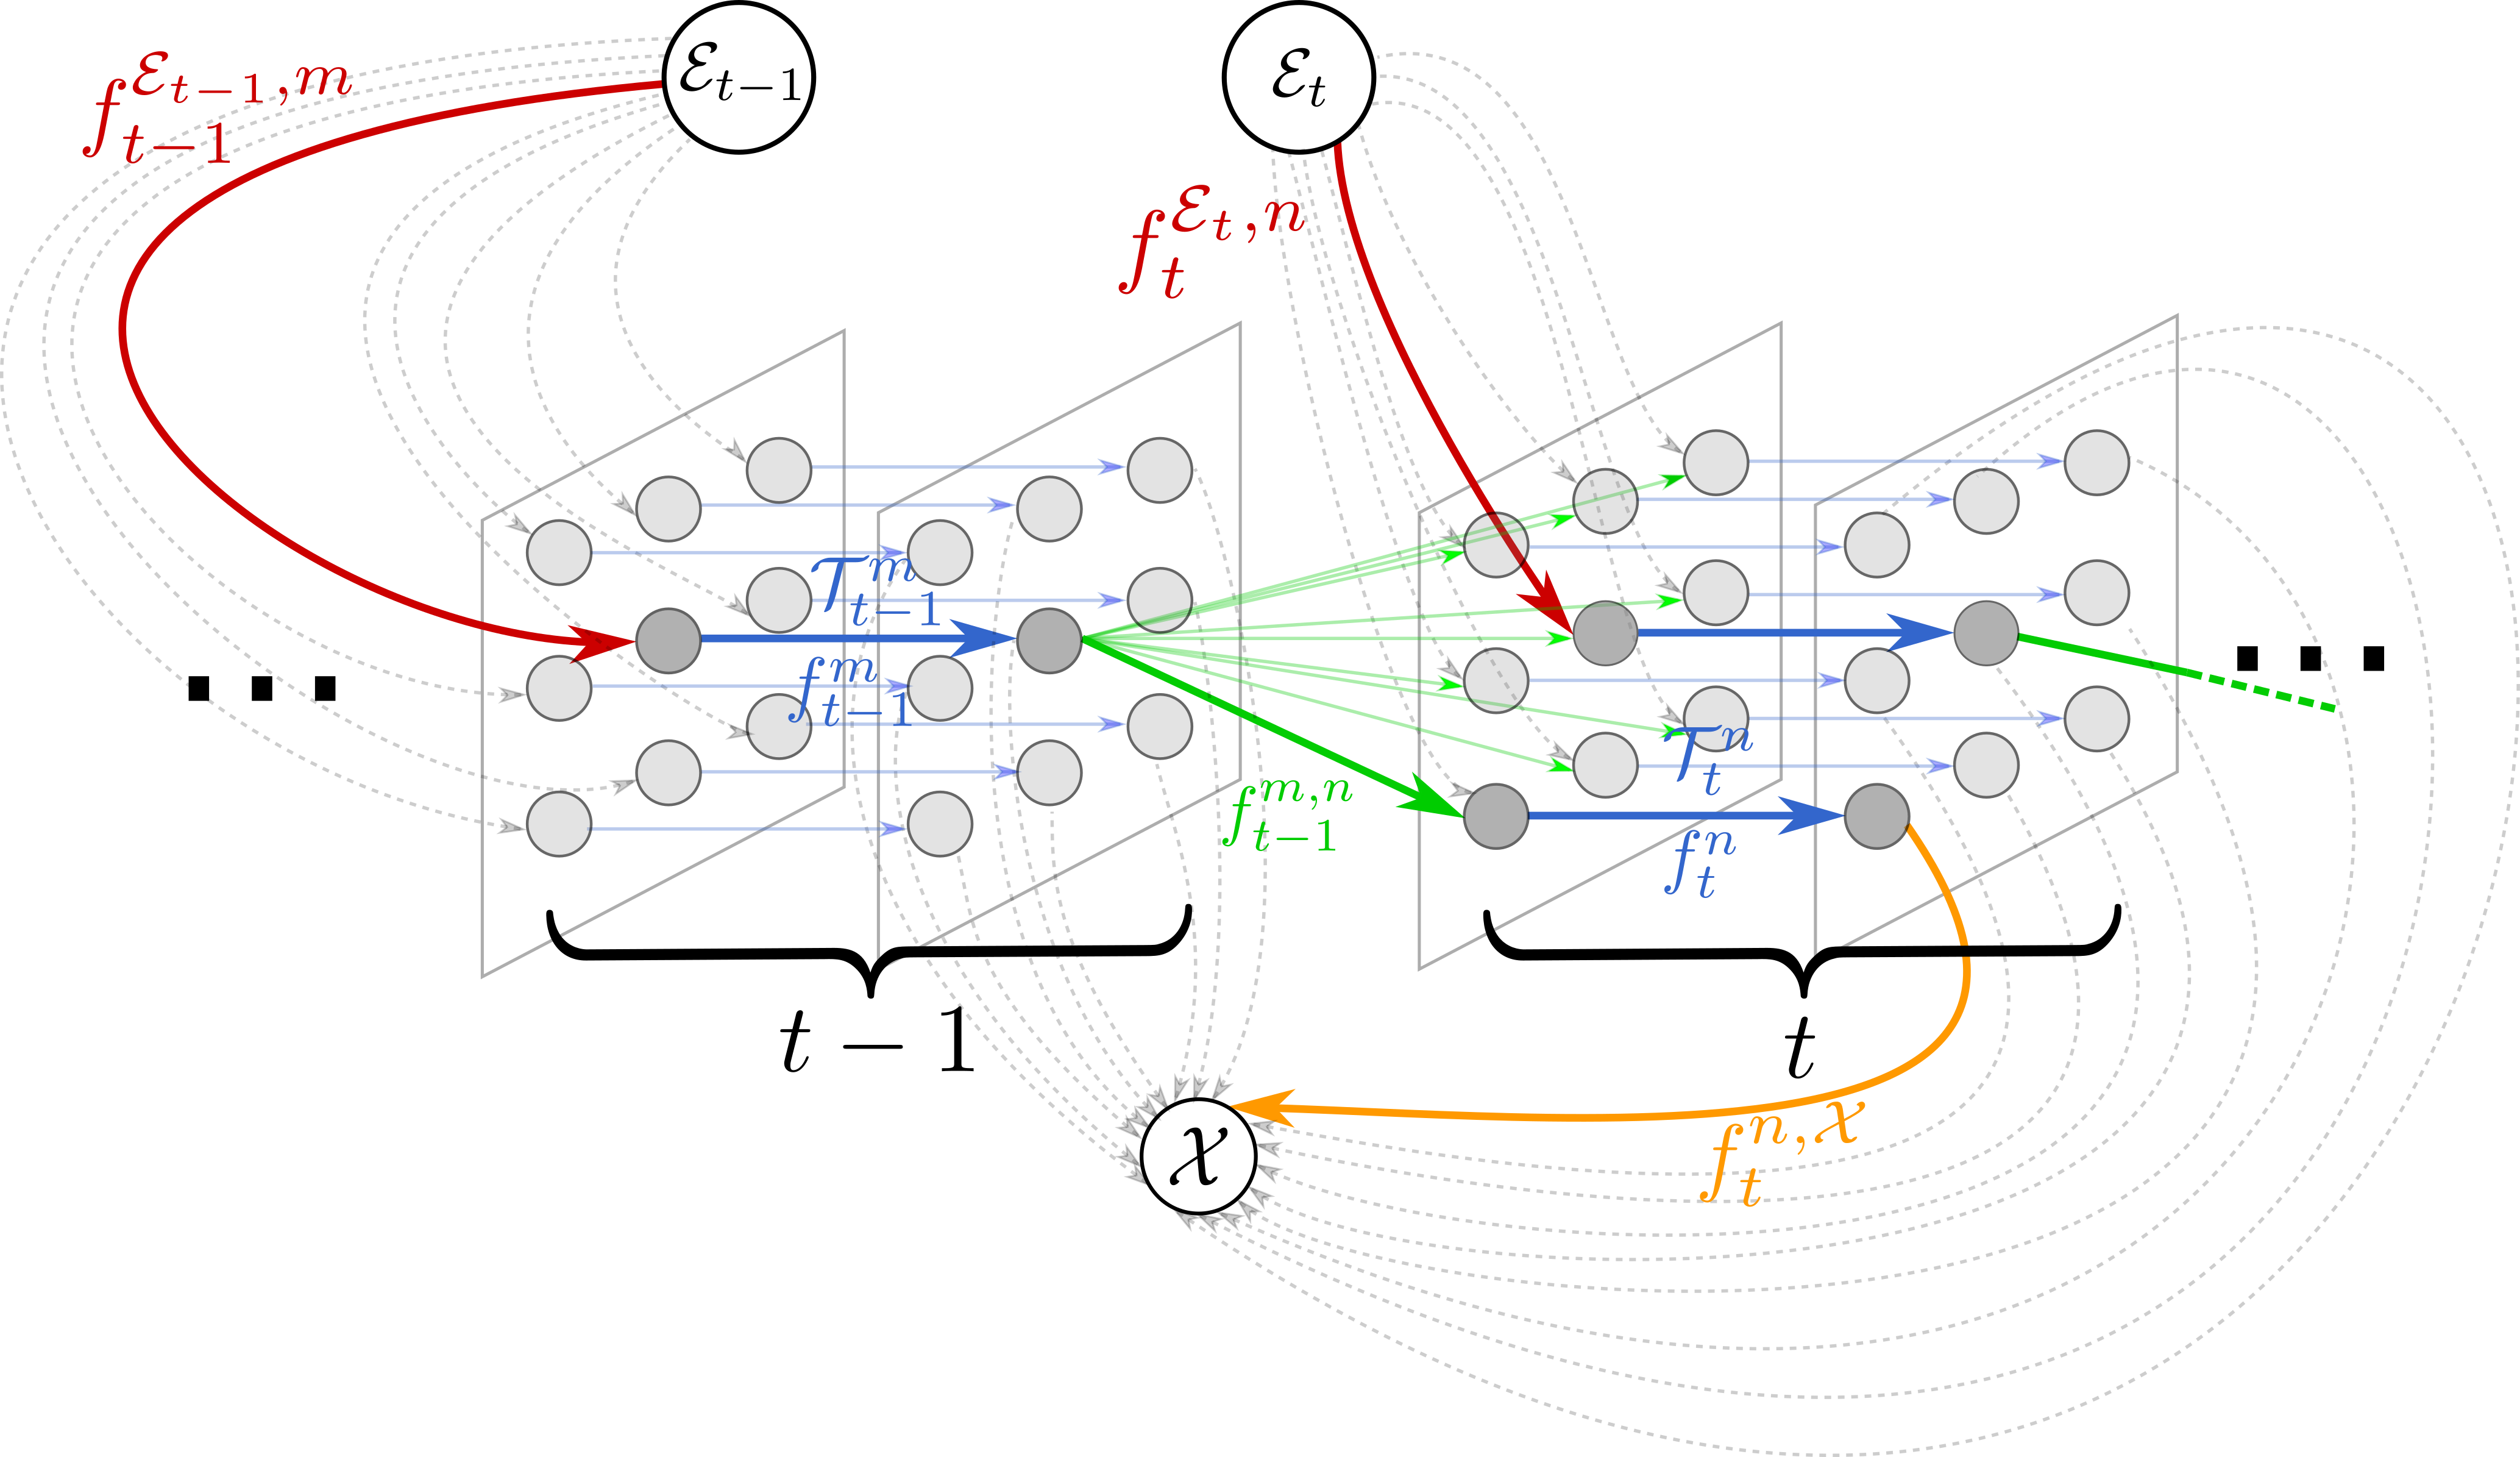
\includegraphics[width=1.\textwidth]{ksp_network}
\caption{Max-Flow graph (forward case). At each time frame $t$, a ``pseudo'' source node $\mathcal{E}_t$ is connected via an edge with flow $f_{t}^{\mathcal{E},n}$ (red) to tracklet $\mathcal{T}_t^n$. Each tracklet incurs a flow $f_t^n$ (blue) to visit superpixel $s_t^n$. Tracklets in frame $t$ are connected to tracklets in the next frame and allow for flows $f_{t}^{m,n}$ (green). The flow $f_{t}^{n,\mathcal{X}}$ can leave any tracklet in the network (orange).}
\label{fig:ksp_network}
\end{figure}

\textbf{Transductive Foreground Model: }
The transductive foreground model quantifies the cost associated with flow visiting a given superpixel, as depicted by the blue edges of Fig. \ref{fig:ksp_network}. Let the image sequence be denoted $\mathcal{I} = \{I_0,\ldots,I_T\}$ and let $\bm{g} = \{g_t\}_{t=0}^T$ with $g_t\in\mathbb{R}^2$ be a given 2D pixel location in $I_t$.
All images are assumed to be pre-segmented with $N$ superpixels $S_t=\{s^n_t\}_{n=0}^{N_t}$ using~\cite{achanta12}.
In addition, each superpixel $s_t^n$ has appearance feature vector $z_t^n$ and $\bm{z}=\{z_t^n | t=0,\ldots,T,\quad n=0,\ldots,N_t\}$ is a set of all such feature vectors over all images.
Denoting the set $\mathcal{S}^p = \{s^n_t | g_t \in s^n_t, t=0,\ldots,T,n=0,\ldots N_t \}$ as all superpixels observed and the rest as $\mathcal{S}^u = \mathcal{S} \setminus \mathcal{S}^p$, as well as $\bm{Y} = \{Y_t^n|\forall(t,n)\}$ as the set of binary random variables such that $Y_t^n=1$ when superpixel $s_t^n$ belongs to the object, and $0$ otherwise. The objectness probability of all superpixels given all attended superpixels, denoted $\rho_{t}^n = P(Y_t^n = 1 | \bm{z}, \bm{g})$, is obtained by fitting a set of decision trees in a P-U learning scheme. This is achieved by averaging the votes of decisions trees.

\textbf{Pairwise Probability Model: }
Given two superpixels $s_t^i$ and $s_{t'}^j$, let $\alpha_{t,t'}^{i,j}$ define the probability that they are similar, whereby establishing a cost of either entering the network or transiting from one frame to the next (\ie depicted by the red and green edges of Fig.~\ref{fig:ksp_network}). In \cite{lejeune18}, $\alpha_{t,t'}^{i,j}$ are obtained via a supervised metric-learning where samples are split in a positive and negative set by thresholding on $\bm{\rho} = \{ \rho_t^n | \forall(t,n)\}$
 and then using Fisher Discriminant Analysis \cite{welling05} to maximize inter-class variance and minimize intra-class variance.

\subsection{A Deep Embedded Clustering Approach}
\label{sec:dec}
While the above methods were shown to be effective, they suffer from the fact (1) that the feature encoding component is decoupled from the similarity metric optimization component and (2) the superpixel similarity measure $\alpha_{t,t'}^{m,n}$ is taken as a simple Gaussian distance in the feature space, which ignores the potential presence of sub-populations (clusters). In the following, we describe our contribution which focuses on modeling of the likelihoods (costs) associated to the red, blue, and green edges of Fig.~\ref{fig:ksp_network}.

Our approach to model these costs is inspired by the Deep Embedded Clustering (DEC)~\cite{xie15} that optimizes for the similarity metric and the feature encoding jointly, and which allows us to leverage a sequence-specific distance between clusters. We now describe in detail our approach which is illustrated in Fig.~\ref{fig:network} and consists of two components: (1) an initial feature learning model that learns a representation and (2) a self-supervised clustering method which allows efficient similarity estimation between image regions. In our approach, both are learned end-to-end.
\begin{figure}[b!]
\centering
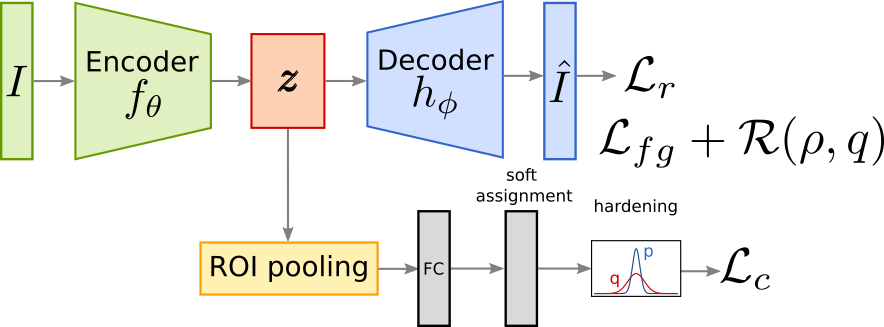
\includegraphics[width=0.79\textwidth]{network2.png}
\caption{The top row is a convolutional neural network configured for autoencoding. Features are pooled on regions of interest (Superpixels) and projected to a low dimensional space via a fully connected layer (FC). The soft assignments $q$ are then optimized to their hardened target assignments $p$.}
\label{fig:network}
\end{figure}

\subsubsection{Feature encoding: }{
  Using a traditional encoder-decoder approach for image reconstruction, our network computes a latent space representation at each pixel.
  Given that our graph operates on a superpixel representation, we use average-pooling on the feature map on all pixels belonging to a superpixel (ROI pooling) and then use a low-dimensional projection, via a fully connected layer, to have a compact representation $z_i$.
}

\subsubsection{Self-supervised clustering: }{ 
We hypothesize that our objects of interest are aggregations of superpixels that potentially span several frames. We assume that a single annotation point is given per frame and wish to train a model that will give a measure of similarity of the given sample with its neighbors. Ideally, we wish to assign  $v_i$ to clusters such that each cluster has low intra-variance. 

Let $\bm{\mu}=\{\mu_j \in V\}_{j=1}^k$ be a set of $k$ centroids lying in the feature space $V$.
Letting $v_i$ the dimensionally reduced feature vector that corresponds to $z_i$, a similarity to centroid $\mu_j$ computed by the student's t-distribution,
\begin{equation}
q_{ij} = \frac{(1 + ||v_i - \mu_j ||^2)^{-1}}{\sum_{j'}(||v_i - \mu_{j'} ||^{2})^{-1}}.
\label{eq:soft_assign}
\end{equation}
}
\noindent
Note that Eq.~\eqref{eq:soft_assign} is a soft version of a typical K-means cluster assignment (\ie $q_{ij}$ are not binary as in K-means). From Eq.~\eqref{eq:soft_assign}, we can derive a target distribution that aims at hardening this t-distribution,
\begin{equation}
p_{ij} = \frac{q_{ij}^2 / f_j}{\sum_{j'}q_{ij'}^2/f_{j'}}
\label{eq:tgt_assign}
\end{equation}
\noindent
where $f_{j}=\sum_i{q_{ij}}$.
Hence, the distribution $p_{i}$ is a more strongly peaked distribution to that of $q_{i}$ and our objective is to learn the centroids $\mu_j$ such that $p_{i}$  and $q_{i}$ are similar to each other, while simultaneously changing $V$ to achieve this.
We detail how to optimize this next.

\subsubsection{Optimization: }{ 
To learn $v_i$ and $\bm{\mu}$, we first use a pre-training phase to optimize a reconstruction loss between the input images $I$ and the reconstructions $\hat{I}$ using a standard encoder-decoder architecture:
\begin{equation}
\mathcal{L}_r = \frac{1}{|I|}\sum_{k,l} ||I(k,l) - \hat{I}(k,l)||^2.
\label{eq:loss_recons}
\end{equation}
\noindent
In a second stage, we use a clustering purity loss that will harden our clusters towards their targets using the Kullback-Leibler divergence:
\begin{equation}
\mathcal{L}_c = D_{KL}(P||Q),
\label{eq:loss_sim}
\end{equation}
\noindent
where $Q$ is a batch of soft-assignments $q_{ij}$ and $P$ the corresponding targets $p_{ij}$.
The complete loss function then optimizes for both cluster purities and the reconstruction loss so as to restrict the distortion of the feature space:
\begin{equation}
\mathcal{L} = \mathcal{L}_c + \gamma \mathcal{L}_r.
\label{eq:loss}
\end{equation}

\subsubsection{Implementation and training: }{ 
  The autoencoder used is a Deeplabv3+ architecture~\cite{chen17} with Dilated Residual Network (DRN) as backbone~\cite{yu17}. 
In contrast with the original architecture, we remove the skip connection that includes the low-level features of the encoder at the input of the decoder. The Deeplabv3 architecture combines the latter output to a dilated spatial pyramid pooling module to extract feature maps in parallel at different spatial scales. By concatenating these, we obtain a feature map that better captures multi-scale context. We use the method described~\cite{schuurmans18} for the ROI pooling module.
  
The autoencoder is pre-trained with data augmentation for $100$ epochs and a learning rate of $10^{-1}$.
In its original formulation, DEC is inherently unstable as all target distributions $\bm{q}$ are modified at each gradient descent iteration \cite{guo17}.
We therefore implement a buffer that stores the targets of all samples before training.
The targets are then updated for all samples every $T=10$ epochs.
Before the clustering phase, we compute the soft-assignment module with $K=15$ centroids using the K-means algorithm.
Likewise, the dimensionality reduction layer is initialized in a similar fashion as~\cite{lejeune18} to $15$ dimensions.
The encoder, decoder, centroids, and fully connected layer are optimized for $200$ epochs with a learning rate $10^{-3}$ and $\gamma=0.1$.
All sequences are pre-segmented into $\sim 1200$ superpixels per-frame.
}

\subsubsection{Clustering-based pairwise probability model: }{ 
Once trained, we use the optimized centroids $\bm{\mu}$ as follows. We assign each sample $v_i$ to a cluster $c_i=\arg \max_{j}q_{ij}$.
We then fit a Gaussian mixture model on all samples by taking as initial means $\bm{\mu}$, component weights $\bm{\pi}=\{\pi_j|\pi_j=|c_j|/N\}$, and covariance matrices $\Sigma_j=cov[\bm{v_j},\bm{v_j}]$. By letting $p(v_i) = \left[ \cdots \pi_j \mathcal{N}(v_i|\mu_j,\Sigma_j)\cdots \right]$ be the posterior probabilities of sample $v_i$, we can then compute the pairwise similarity of $v_i$ and $v_{i'}$ as the Bhattacharya coefficient of $p(v_i)$ and $p(v_{i'})$,
\begin{equation}
BC_{ii'} = \sum_{k=1}^K{\sqrt{p(v_i)_k p(v_{i'})_k}}.
\label{eq:bc}
\end{equation}
}
\noindent
Eq.~\eqref{eq:bc} thus provides the costs associated to the green and red edges in Fig.~\ref{fig:ksp_network}.
%%% Local Variables:
%%% mode: latex
%%% TeX-master: "00_main"
%%% End:

\section{Experiments}
\label{sec:experiments}

\subsection{Datasets and baselines}
\label{sec:data}
To validate our method, we evaluate its performance on the publicly available dataset used in~\cite{lejeune18}. This consists several video and volumes of different modalities with 2D annotation points for different object types. Briefly, it includes:
\begin{itemize}
\item[-]{\bf{Brain:}} $4$ 3D T2-weighted MRI scans from the publicly available BRATS challenge dataset~\cite{menze15}, where tumors are object of interest
\item[-]{\bf{Tweezer:}} $4$ sequences from the training set of the publicly dataset MICCAI Endoscopic Vision challenge: Robotic Instruments segmentation~\cite{endochal}. The piecewise-rigid surgical instrument must be segmented.
  
\item[-]{\bf{Slitlamp:}} $4$ slit-lamp video recordings of human retinas, where the optic disk is to be segmented. 

\item[-]{\bf{Cochlea:}} $4$ volumes of 3D CT scans of the inner ear, where the cochlea must be annotated. This object is the most challenging object to segment due to its complicated geometry. 
\end{itemize}

To this, we evaluate the following methods:
\begin{itemize}
\item[-]{\bf Gaze2Segment:} A combination of saliency detection and graphcut~\cite{khosravan16}. 
\item[-]{\bf DL-prior:} Point location supervision is used to train a CNN with strong object priors~\cite{bearman16}.
\item[-]{\bf EEL:} An expected exponential loss to learn robust classifiers in a PU learning setting~\cite{lejeune17}. 
\item[-]{\bf KSPTrack:} Multiple-instance tracking method described in~\cite{lejeune18}. 
\item[-]{\bf KSPTrack/GMM:} Our approach with entrance and transition costs computed according to Eq.~\eqref{eq:bc}.
\item[-]{\bf KSPTrack/DEC} Our approach using the proposed Deep Embedded Clustering described above.
\end{itemize}

\subsection{Experiments}
\subsubsection{Accuracy of segmentations}
Table \ref{tab:results} shows on each baseline the F1 score between the generated segmentation and the corresponding groundtruth annotation.
Figure \ref{fig:qualitative} shows for each sequence type graphical example.
Note that our clustering approach tends to improve the foreground probability maps (second vs. fifth column).

\begin{table}
\centering
\caption{
Quantitative results on all datasets. We report the F1 scores and standard deviations.
}
\label{tab:results}
\begin{tabular}{llp{1.8cm}p{1.8cm}p{1.8cm}p{1.8cm}p{1.8cm}}
\toprule
Types &                 Brain &               Cochlea &              Slitlamp &              Tweezer \\
Methods      &                       &                       &                       &                      \\
\midrule
KSPTrack/DEC &  $\bm{0.83} \pm 0.03$ &        $0.58 \pm 0.1$ &       $0.72 \pm 0.08$ &  $\bm{0.79} \pm 0.1$ \\
KSPTrack/GMM &       $0.82 \pm 0.04$ &        $0.58 \pm 0.1$ &        $0.72 \pm 0.1$ &      $0.78 \pm 0.09$ \\
\hdashline
KSPTrack     &       $0.74 \pm 0.08$ &  $\bm{0.66} \pm 0.02$ &  $\bm{0.77} \pm 0.08$ &      $0.77 \pm 0.08$ \\
EEL          &       $0.52 \pm 0.14$ &       $0.12 \pm 0.05$ &       $0.59 \pm 0.08$ &       $0.6 \pm 0.16$ \\
Gaze2Segment &       $0.07 \pm 0.02$ &       $0.07 \pm 0.02$ &        $0.02 \pm 0.0$ &       $0.18 \pm 0.0$ \\
DL-prior     &       $0.56 \pm 0.08$ &        $0.3 \pm 0.04$ &       $0.51 \pm 0.11$ &      $0.72 \pm 0.06$ \\
\bottomrule
\end{tabular}
\end{table}


\begin{figure}[h!]
\centering
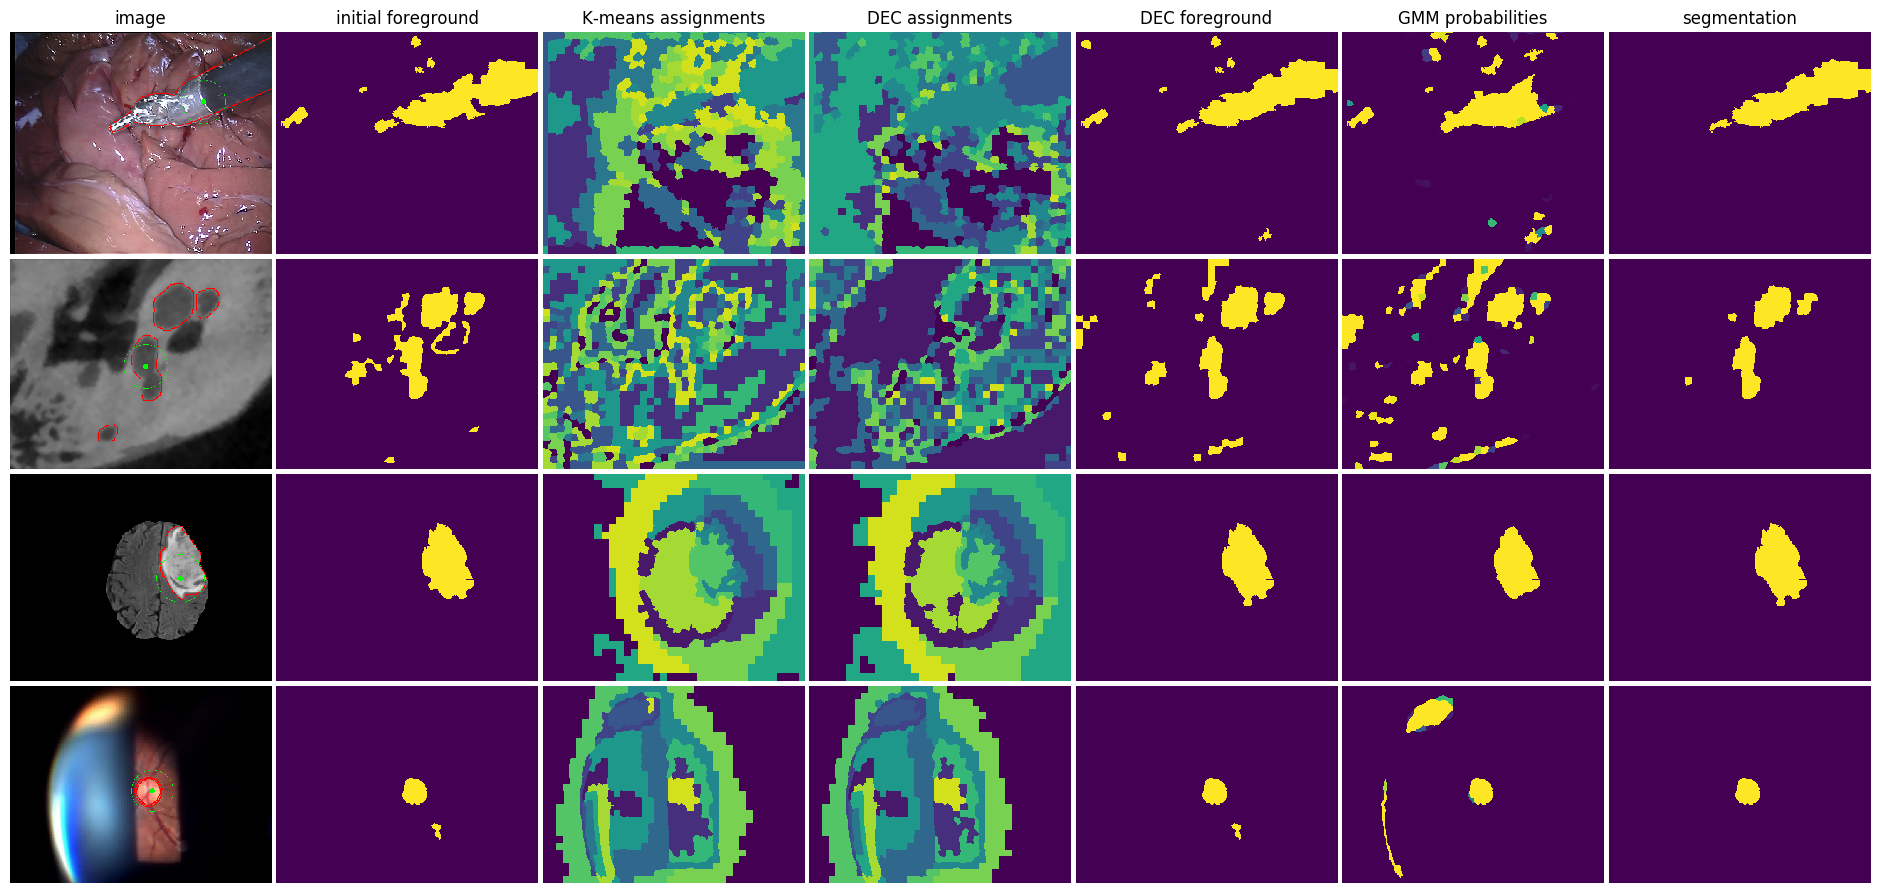
\includegraphics[width=1.\textwidth]{prevs}
\caption{Qualitative results showing from left to right: (1) Original frame with ground truth contour in red and 2D location in green. The entrance region is the outer circle (2) Thresholded foreground probabilities using plain autoencoder's features. (3) Clusters from K-means. (4) Clusters after DEC. (5) Thresholded foreground probabilities with optimal features. (6) Entrance probabilities given user input of column 1. (7) Final segmentation}
\label{fig:qualitative}
\end{figure}


%%% Local Variables:
%%% mode: latex
%%% TeX-master: "../../main"
%%% End:

\section{Conclusion}
\label{sec:conclusion}

We presented a framework that allows pixel-wise segmentation of medical sequences based on minimal point-wise supervision.
Using a self-supervised clustering approach, features of superpixels were learned so as to minimize a purity measure.
We evaluate on a number of different medical datasets, with several inherent difficulties.
The results show that the addition of the clustering task can in some cases help the sparse point segmentation task.
However, we noticed that through the clustering process, the reconstruction and clustering objectives come into conflict, i.e the entrance/transition model gets better as the foreground model gets worse, thereby having a detrimental effect on performance.
The observed variance between the different sequences of the same type can be explained by the fact that in some cases, where one of the four sequences is noisier than the others, the k means clustering encounters limitations, that are reflected both to the mean and the variance.

We conclude by emphasizing on the flaws and learned lessons of the proposed approach:
First, \gls{dec} is not suited to our application since it does not explicitely leverages spatial/temporal relations between samples in the learning process.
We made several attempts at optimizing pairwise constraints along with the clustering purity criteria, but found that the learning process became unstable.
Second, the foreground prediction is not an explicit part of the learning algorithm, but is rather an ad-hoc component that is meant to benefit from better features.
We consider this a strategic flaw since \gls{cnn}s are known to perform well on segmentation/prediction tasks.
In particular, a \gls{cnn} configured for a segmentation task would optimize for both features and classifier function.
On a more positive note, this work was an opportunity to explore a rich field of machine learning: Self-supervised learning.
In the next chapter, we therefore conserve the idea of self-supervision and devise a positive-unlabeled learning method coupled with a strategy to augment the set of positive superpixels.

%%% Local Variables:
%%% mode: latex
%%% TeX-master: "00_main"
%%% End:


%%% Local Variables:
%%% mode: latex
%%% TeX-master: "../../main"
%%% End:
